%----------------------------------------------------------------------------------------
%	PACKAGES AND DOCUMENT CONFIGURATIONS
%----------------------------------------------------------------------------------------

\documentclass{article}

\usepackage[italian, english]{babel}	% lingua principale inglese con alcune parti in italiano
\usepackage[version=3]{mhchem} % Package for chemical equation typesetting
\usepackage{siunitx} % Provides the \SI{}{} and \si{} command for typesetting SI units
\usepackage{graphicx} % Required for the inclusion of images
\usepackage{natbib} % Required to change bibliography style to APA
\usepackage{amsmath} % Required for some math elements 
\usepackage[utf8]{inputenc}
\usepackage[italian, english]{babel}	% lingua principale inglese con alcune parti in italiano
\usepackage{newlfont}					% codifica il font
\usepackage{color}
\textwidth=450pt\oddsidemargin=0pt

\usepackage{booktabs}					% include tabelle
\usepackage{caption}
\usepackage{graphicx}					% include le figure
\usepackage{float}
\usepackage{subfigure}						% figure multiple

\renewcommand{\varepsilon}{\epsilon}    % convenzione sulle lettere
\renewcommand{\vartheta}{\thetha}		% greche da usare
\renewcommand{\varrho}{\rho}
\renewcommand{\varphi}{\phi}

\usepackage{amsmath}					% pacchetti matematici
\usepackage{amssymb}
\usepackage{amsfonts}
\usepackage{mathptmx}

\setlength{\parindent}{0.5cm}

\renewcommand{\thefootnote}{\fnsymbol{footnote}} % poche note a pie' pagina

%\setlength\parindent{0pt} % Removes all indentation from paragraphs

\renewcommand{\labelenumi}{\alph{enumi}.} % Make numbering in the enumerate environment by letter rather than number (e.g. section 6)

%\usepackage{times} % Uncomment to use the Times New Roman font

%----------------------------------------------------------------------------------------
%	DOCUMENT INFORMATION
%----------------------------------------------------------------------------------------

\title{
  \huge{\textbf{An FPGA Implementation of a\\ Deep Autoencoder using hls4ml package \\}}
  \Large{\textsc{\\ Alma Mater Studiorum $\cdot$ University of Bologna \\ }}
  \large{\textsc{Department of Physics and Astronomy \\}}
  \normalsize{\textsc{Applied Electronics course}}
  } % Title

\author{Lorenzo Valente} % Author name
  
\date{\today} % Date for the report

\begin{document}

\maketitle % Insert the title, author and date

\begin{center}
\begin{tabular}{l r}
%Date Performed: & December -, 2021 \\ % Date the experiment was performed
%Partners: & James Smith \\ % Partner names
%& Mary Smith \\
%Instructor: & Professor Smith % Instructor/supervisor
\end{tabular}
\end{center}

% If you wish to include an abstract, uncomment the lines below
% \begin{abstract}
% Abstract text
% \end{abstract}


\section*{\centering{Abstract}}
In this report is presented an implementation of a \textit{Deep Autoencoder} 
architecture trained on the MNIST database in FPGA (Field Programmable Gate Array), 
focusing on machine vision tasks for the data reconstruction and classification in the latent dimension.
To implement machine learning (ML) models in FPGAs, a companion compiler 
based on High-Level Synthesis (HLS) called hls4ml is used. 

%----------------------------------------------------------------------------------------
%	SECTION 1
%----------------------------------------------------------------------------------------

\section{Introduction}


\begin{figure}[H]
  \centering
  \includegraphics[scale=0.17]{images/section1/overview.jpg}
  \caption{A typical workflow to translate a model into an FPGA implementation using hls4ml.}
  \label{fig:overview}
\end{figure}


The hls4ml package was developed by members of the High Energy Physics (HEP) community
to translate ML algorithms into HLS code, enabling firmware development times to be drastically reduced.
In this project development, hls4ml is used as the tool to perform 
this transformation on a trained Deep Autoencoder model.
A schematic workflow is shown in figure \ref{fig:overview}.

\par The goal of the hls4ml package is to empower a HEP physicist to accelerate
ML algorithms use FPGAs, thanks to their tools for the conversion. 
Indeed, hls4ml translates Python objects into HLS, and its
synthesis automatic workflow, allowing fast deployment times also for
those who know how to write software or are not yet experts on FPGAs.



%----------------------------------------------------------------------------------------
%	SECTION 2
%----------------------------------------------------------------------------------------

\section{Data preparation}
The first important step before model creation is data preparation.
\par Vivado HLS capabilities enable to generate hls4ml's cores with 
at most 4096 parameters calculation, i.e. 12 bit, for each neural network's layer. 
Considering this constraint, as well as the consistency of the model's output,
a reduction in the input image resolution is performed on the original datasets. 

\begin{figure}[H]
  \centering
  \begin{minipage}[c]{.4\textwidth}
   {\includegraphics[scale=0.7]{images/section1/original_data.png}}
    \end{minipage}
    \qquad \qquad
      \begin{minipage}[c]{0.4\textwidth}
  {\includegraphics[scale=0.7]{images/section1/modified_data.png}}
     \end{minipage}
     \quad
     
   \caption{On the \textit{left} an image from the original dataset.
   On the \textit{right} the modified dataset after the preprocessing.}
    \label{fig:MNIST}
\end{figure}

\par The MNIST database is chosen as input for our model.
The original database contains handwritten digits, from 0 to 9. 
MNIST has been divided into two datasets: the training set has 60,000 samples and the test set has 10,000.
Each image contains a single handwritten digit, each one with 28x28 pixels 
ranging from 0 to 255, i.e. 8-bit grayscale value.
\par In particular, the preprocessing that we performed on the original MNIST database consists of:
\begin{itemize}
    \item \textbf{cropping the central portion} from size 28x28 to 22x22 pixels;
    \item \textbf{downsampling} for reducing the resolution from 22x22 to 8x8 pixels;
    \item \textbf{transforming of the color depth} from 8-bit to 5-bit.
\end{itemize}

The last point is chosen simply for reasons of hardware capability.
The images in figure \ref{fig:MNIST} are shown as an example, the first image from the original training dataset
and the same figure after the preprocessing.



%----------------------------------------------------------------------------------------
%	SECTION 3
%----------------------------------------------------------------------------------------
\section{Choosing the Model}
\textit{Autoencoding} is a data compression algorithm, where the compression (\textit{encoding}) and decompression (\textit{decoding}) functions are:
\begin{itemize}
  \item \textbf{data-specific}, therefore they will only be able to compress data similar to what they have been trained on;
  \item \textbf{lossy}, which means that the decompressed outputs will be degraded compared to the original inputs;
  \item \textbf{learned automatically from data examples}, it means that it is easy to train specialised instances of the algorithm, 
          that will perform well on a specific type of input.
\end{itemize}

\par The design of a \textbf{deep fully-connected autoencoder} implemented uses an architecture which imposes a \textit{bottleneck} on the network. 
It forces a compressed knowledge representation of the input data.
In this implementation, it is used compression in \textit{two-dimensional} latent space. 
Compression and reconstruction are extremely demanding if there is no structure in the data, 
i.e. no correlation between input features. 
However, if some sort of structure exists in the data, it can be learned and applied when forcing the input through the bottleneck.
The model has been considered both with and without the classifier for the decompression.

\subsection{Autoencoder for the Reconstruction}
After some experimentation with different node sizes, considering the consistency of 
the algorithm's output as well, we find an optimal structure for each layer as depicted in figure \ref{fig:ae}. 

\begin{figure}[H]
  \centering
  \includegraphics[scale=0.4]{images/section3/autoencoder_reco.png}
  \caption{Implemented autoencoder model. The \textbf{encoder} (\textit{left part}) takes 64 nodes in input layer, 32 and 16 nodes for
  hidden layers respectively ending up into a compressed two-dimensional latent space. 
  The \textbf{decoder} (\textit{right part}) takes as input the two-dimensional latent space and decompress the information 
  in complete ascending analogy as the previous encoder structure, ending up into a 64 nodes layer as output.}
  \label{fig:ae}
  \end{figure}

\par The loss function used to train an under complete autoencoder is called \textit{reconstruction loss},
as it is a check of how well the image has been reconstructed from the input.
Although the reconstruction loss can be anything depending on the input and output,
we will use an L1 loss to depict the term represented by the equation (\ref{eq:loss}):

\begin{equation}
  L ( r, \hat{r} ) = | r - \hat{r} |,
  \label{eq:loss} 
\end{equation}
where $r$ is the ground truth and $\hat{r}$ represents the predicted output.

\par All the layer nodes are activated by the \textit{ReLU} function, 
except for the last output layer which is activated by the \textit{sigmoid} function. 



\subsection{Classifier}

To evaluate the correct reconstruction performed by the autoencoder's reconstruction, a classifier has been implemented.
\par The neural networks architecture, shown in figure \ref{fig:classifier}, is attached to the encoder part in the two-dimensional
latent space and it works in parallel with the decoder for the decompression. 
In contrast with the previous architecture, we are now focusing on the classification problem. 
Therefore, for the output layer, the activation function \textit{softmax} is used, so we can train the model exploiting 
the knowledge on the labels from the input datasets.

\begin{figure}[H]
  \centering
  \includegraphics[scale=0.35]{images/section3/autoencoder_classifier.png}
  \caption{Implemented classifier model. It takes as input the compressed space by encoder
  and decompress the information with two hidden layers of 16 and 32 nodes respectively. 
  Ending up with a 10 nodes output layer, one for each digit classification.}
  \label{fig:classifier}
  \end{figure}

  %----------------------------------------------------------------------------------------
%	SECTION 4
%----------------------------------------------------------------------------------------
\section{Neural Network optimization via Compression}

The final hardware platform where the inference computation will run must be considered when building a neural network model. 
To minimize the resource utilization when a neural network is targetted to FPGA, 
aimed at reducing the number of parameters and operations involved in the computation, 
by removing connections and thus parameters.

\par This process is commonly called \textbf{weight pruning}, i.e. the elimination of unnecessary values in the weight tensor, 
by practically setting the parameters' values to zero, which will be translated in cutting connections between nodes 
during the synthesis of the HLS design. 
The pruning is done during the training process to allow the NN to adapt to the changes.

\par The TensorFlow Sparsity Pruning API was selected to perform this optimization.
It uses an algorithm designed to iteratively remove connections, based on their magnitude during training.
Therefore, a final target sparsity, i.e. target percentage of weights equal to zero is specified,
along with a schedule to perform the pruning. 
For our experiment, we start pruning at step 2000, stop at step 10000 and do it every 100 steps.
As training proceeds, the pruning routing is scheduled to execute, removing the weights with the lowest magnitude, 
until the current sparsity target is reached.

\subsection{Neural Network model performance on CPU}

\par Pruning a model can harm accuracy. 
To obtain the best accuracy for our model, we explored the trade-off between accuracy, speed and model size.
Therefore, we avoid pruning the first layer and the critical layers for compression and decompression of the information.
We proceeded to prune only the hidden layer with 16 nodes in both compression and decompression parts, we reached a sparsity of 80\%. 
In the figure \ref{fig:weights} are shown the distributions of the weights through the layers.
It can be noticed that in the histograms for the \textit{second}, \textit{fourth} and \textit{fifth} layer we observe large peak in the bin containing '$0$'.

\begin{figure}[H]
  \centering
  \includegraphics[scale=0.5]{images/section4/weights/bitmap.png}
  \caption{Weights distributions of the pruned model with classifier.}
  \label{fig:weights}
\end{figure}

Summary of the pruning technique in the tab \ref{tab:params}. 
As we can see, we reached a reduction in the total number of parameters of almost 0.93\%.

\begin{table} [H]
  \centering
  \begin{tabular}{| c | c | c |}
  
  \hline
  & Complete model  &   Pruned model  \\
  \hline 
  \hline
  $2^{nd}$ layer & 512 + 16 & 102 + 16 \\ %512-102=410
  \hline
  $4^{th}$ layer & 32 + 16 & 6 + 13 \\ %28
  \hline
  $5^{th}$ layer & 32 + 16 & 6 + 15  \\ %25
  \hline
  \textbf{Total parameters} & \textbf{6268} & \textbf{5805} \\
  \hline
  \end{tabular}
  \caption{Results of the pruning technique for the model with classifier.
  There is a complete list of parameters before and after pruning in the format \textit{weight + bias}.}
  \label{tab:params}
\end{table} 

Plotted below are model score losses and classifier accuracies. 
The model has been considered both with without the classifier for the decompression.
Model score losses, computed according to the equation \ref{eq:loss}, approach zero at high epochs as expected.
As it can be noticed, bumps appear near the eighth epoch, meaning that the algorithm for iteratively removing network connection start work.

\begin{figure}[H]
  \centering
  \begin{minipage}[c]{.4\textwidth}
   {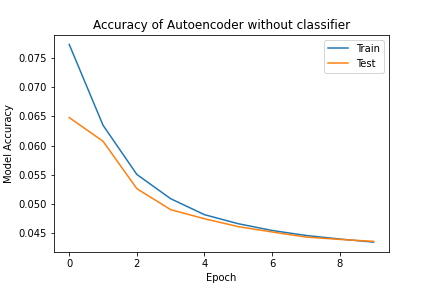
\includegraphics[scale=0.4]{images/section4/AE/Accuracy of Autoencoder without classifier.png}}
    \end{minipage}
    \qquad \qquad
      \begin{minipage}[c]{0.4\textwidth}
  {\includegraphics[scale=0.4]{images/section4/AE/Accuracy of Autoencoder with classifier.png}}
     \end{minipage}
     \quad
  
     \begin{minipage}[c]{0.4\textwidth}
  {\includegraphics[scale=0.4]{images/section4/AE/Accuracy of compressed AE without classifier.png}}
  \end{minipage}
  \qquad \qquad
  \begin{minipage}[c]{0.4\textwidth}
    {\includegraphics[scale=0.4]{images/section4/AE/Accuracy of compressed AE with classifier.png}}
  \end{minipage}
  \quad
     
   \caption{On the \textit{left} an image from the original dataset.
   On the \textit{right} the modified dataset after the preprocessing.}
    \label{fig:accuracy}
\end{figure}

In the following table \ref{tab:results}, we show a summary of performances after a training phase of 30 epochs.
Accuracies and losses do not suffer so much from the pruning procedure.

\begin{table} [H]
  \centering
  \begin{tabular}{| c | c | c |}
  \hline
   & Complete model  &   Pruned model  \\
  \hline 
  \hline
  Training loss & 0.0626 & 0.0668 \\
  \hline
  Testing loss & 0.0628 & 0.0669 \\ 
  \hline
  Training accuracy & 0.9041 & 0.8863 \\ 
  \hline
  Testing accuracy & 0.9020 & 0.8897 \\
  \hline
  \end{tabular}
  \caption{Final results of the performances for pruned and complete model with classifier.}
  \label{tab:results}
\end{table}

Plotted below is the distribution of labelled data in its two-latent dimension space.
In the latent space, it can be noticed a linear distribution of images. 
Each of these coloured clusters is a type of digit. 
Close clusters are structurally similar digits, i.e. digits that share information in the latent space. 
This particular linear distribution describes the fact that we have two dimensions to express a handwritten digit. 
Then it could happen for certain digits that the height increases and the width increase as well, creating a linear shape in the latent space, as displayed. 

\begin{figure}[H]
  \centering
  \begin{minipage}[c]{.4\textwidth}
   {\includegraphics[scale=0.35]{images/section4/AE/Latent dimension of Autoencoder with classifier.png}}
    \end{minipage}
    \qquad \qquad
      \begin{minipage}[c]{0.4\textwidth}
  {\includegraphics[scale=0.35]{images/section4/AE/Latent dimension of Compressed AE with classifier.png}}
     \end{minipage}
     \quad   
   \caption{Digit distributions in the latent space for the model with classifier.}
    \label{fig:latent}
\end{figure}

The last two images of this section represent the original training dataset on the first row and 
for the second row, the reconstructed images after both the complete and pruned model are applied.

\begin{figure}[H]
  \centering
  \begin{minipage}[c]{.4\textwidth}
   {\includegraphics[scale=0.35]{images/section4/AE/reconstructed images complete.png}}
    \end{minipage}
    \qquad \qquad
      \begin{minipage}[c]{0.4\textwidth}
  {\includegraphics[scale=0.35]{images/section4/AE/reconstructed images compressed.png}}
     \end{minipage}
     \quad   
   \caption{Reconstructed images.}
    \label{fig:reco}
\end{figure}

\par The models trained in the previous section were saved into HDF5 files, containing:
\begin{itemize}
  \item the architecture of the model, to be reproduced when it is needed to be used with other datasets;
  \item the model weights;
  \item the training configuration (losses, optimizers);
  \item the state of the optimizer, allowing to resume training exactly where it was left.
\end{itemize}

%----------------------------------------------------------------------------------------
%	SECTION 5
%----------------------------------------------------------------------------------------

\section{FPGA Implementation}
\subsection{Laboratory Implementation}



%----------------------------------------------------------------------------------------
%	SECTION 4
%----------------------------------------------------------------------------------------

\section{Experimental Results and discussion}




%----------------------------------------------------------------------------------------
%	CONCLUSIONS
%----------------------------------------------------------------------------------------

\section{Conclusions}






%----------------------------------------------------------------------------------------
%	BIBLIOGRAPHY
%----------------------------------------------------------------------------------------



\end{document}